\documentclass{article}
  \parindent = 0mm % Sin sangría
  \usepackage[utf8]{inputenc}
  \usepackage[T1]{fontenc}
  \usepackage[spanish]{babel}
  \usepackage{graphicx}
  \usepackage{amstext}
  \usepackage{amsmath}
  \usepackage{booktabs}
  \usepackage{subfigure}
  \usepackage{footnote}
  \usepackage{hyperref}
  \usepackage{algpseudocode,algorithm,algorithmicx}
  \usepackage[font=small,labelfont=bf]{caption}

\begin{document}
  \begin{center}
    {\sc \large Metaheurístcas y optimización sobre redes}
    
    {\sc \large Obligatorio 2020}
    \linebreak

    {\rm Joaquín Correa - \today}
  \end{center}

  \section*{Introducción}

  En este documento se presenta un GRASP como metaheurístca para el problema de ruteo de vehículos (VRP) con ventanas de tiempo y flota heterogénea, basandose en el modelo fomulado por (\ref{inco}) y en los modelos y resultados de problemas similares estudiados por Solomon (\ref{solomon}) y Jiang (\ref{jiang}).

  El GRASP desarrollado permite encontontrar soluciones a estos modelos siendo estas en algunos casos muy cercanas al óptimo.

  \section*{Problema}

  El problema que se quiere resolver es un clásico VRP con el adicionado de ventanas flexibles, esto quiere decir que los vehiculos pueden atender los clientes luego de finalizada la ventana de tiempo pagando cierta penalidad. Considerar esto es de utilidad ya que pueden encontontrarse soluciones cuyo costo es significativamente menor al de un VRP con ventana fija y puede tener sentido práctico en ciertos contextos.

  \subsection*{Representación}

  Para la representación del problema en computadora se requiere:
  
  \begin{itemize}
    \item Una matriz de distancia entre clientes $t_{ij}$. La distancia está expresada en unidades de tiempo.
    \item Una lista de vehículos, cada vehículo $v$ con un costo fijo $f_v$, costo variable $\alpha_v$ y capacidad $q_v$.
    \item Una lista de clientes. Cada cliente $i$ cada uno con una demanda $d_i$, un tiempo de servicio $s_i$ y un rango de tiempo $e_i, l_i$ que representan el tiempo mínimo y máximo en que puede llegar un vehículo.
    \item Un nodo origen, desde el que salen y llegan los vehículos. Se modela como un cliente con demanda 0.
    \item Un porcentaje de flexibilidad de la ventana de tiempo de los clinetes $w$. Es decir un valor que permite que el arribo a un cliente $i$en cualquier momento dentro de $[e_i, l_i + (l_i - e_i)w]$ sea factible.
    \item Un parámetro $\rho$ de penalización por arribo a los clientes luego del valor $l_i$.
  \end{itemize}

  \section*{Metaheurístca}

  TODO: Por que elegí GRASP

  \section*{GRASP}
  
  El GRASP implementado es una versión estándar que tiene las siguientes características:

  \begin{description}
    \item[RCL de tamaño variable parametrizada por $\alpha$:] La RCL es una lista de candidatos $m_i$ con costo asociado $c_i$ que cumplen que $c_i \in [c_{min}, min + (c_{max} - c_{min}) \alpha]$
    \item[Búsqueda local múltiple:] Durante la fáse de búsqueda local se recorren dos tipos de vecindades.
  \end{description}

  El algorítmo seguido se detalla en el pseudocódigo (\ref{grasp}).

  \begin{algorithm}
    \begin{algorithmic}
      \Function{Grasp}{$instance$}
        \State{$bestSol \longleftarrow Null$}
        \For{$iter \in 0..MaxIter$}
          \State{$sol \longleftarrow ConstructSolution(instance)$}
          \If{$sol == Null$}
            \State{$continue$}
          \EndIf
          \For{$localSearchIter \in 0..LocalSearchMaxiter$}
            \State{$sol \longleftarrow LocalSearch(instasnce, sol)$}
              \If{$hasImproved(sol)$}
              \State{break}
            \EndIf
          \EndFor
          \If{$value(sol) < value(bestSol)$}
            \State{$bestSol \longleftarrow sol$}
          \EndIf
        \EndFor
        \State \Return $bestSol$
      \EndFunction
    \end{algorithmic}
    \caption{Algorítmo GRASP \label{grasp}}
  \end{algorithm}

  El desarrollo y ajuste de parámetros se realizó ejecutando 18 de las instancias del dataset Solomon de 25 nodos para las cuales se tienen valores óptimos o muy buenos de soluciones tanto para ventana fija como para ventana flexible.

  \subsection*{Fase de construcción}

  Esta fase, representada por la función $ConstructSolution(instance)$ en el pseudocódigo (\ref{grasp}), construye una solución a partir de un conjunto de rutas inicialmente vacías. Una ruta representa el recorrido de un vehículo. En cada iteración se decide un movimiento de vehículo a cliente y por lo tanto se agrega el cliente a la ruta asociada al vehículo. De esta manera se construyen potencialmente varias rutas de manera simultánea.

  El procedimiento seguido en cada iteración es: para cada vehículo se toman los $MovesPerVehicle$ mejores movimientos posibles, de entre los factibles, y se agregan a una lista, luego se construye la RCL a partir de dicha lista de movimientos. Vale la pena aclarar que se consideran todos los vehículos, incluso los que no tienen clientes asignados y se asume que se encuentran en el nodo origen.

  Los mejores movimientos son determinado por su costo. El costo de un movimiento depende del cliente actual en que se encuentra el vehículo, el cliente destino y el tiempo corriente para el vehículo. De esta manera se computa el costo del vehículo $v$, desde el cliente $i$ al cliente $j$ en tiempo $T_v$ como:

  \begin{align}
    CostoMov(v, i, j, T_v) = W_d t_{ij} + W_t PT_{ij}^{T_v} + W_w WT_{ij}^{T_v} + OT_{ij}^{T_v} \rho + \beta_i
    \label{eq:rclmovecost}
  \end{align}
  
  Donde, sea $a_{vj} = T_v + t_{ij}$ el momento de arribo a del vehículo $v$ al cliente $j$:
  \begin{description}
    \item[$i, j$:] Son los clientes desde y cliente hasta para los que quiero evaluar el movimiento.
    \item[$T_v$]: Es el corriente para el vehículo $v$.
    \item[$W_d, W_t, W_w$:] Son pesos constantes configurables.
    \item[$PT_{ij}^{T_v}$:] Es la diferencia de tiempo desde el arribo a $j$ hasta el momento de cierre $l_j$. Es decir $max(l_j - a_{vj}, 0)$.
    \item[$WT_{ij}^{T_v}$]: Es el tiempo de espera hasta la apertura de $j$. Es decir $max(e_j - a_{vj}, 0)$. Consideramos que es factible que un vehículo arribe a un cliente antes de su momento de apertura, caso en el cuál debe esperar hasta la apertura.
    \item[$OT_{ij}^{T_v}$:] Es el {\it overtime}, o tiempo excedido de arribo luego del cierre de $j$. Es decir $max(a_{vj} - l_j, 0)$.
    \item[$\beta_v$]: Parámetro que vale el costo fijo $f_v$ si $i$ es el nodo origen y $0$ sino.
  \end{description}

  La idea de los parámetros $PT_{ij^{T_v}}$ y $WT_{ij^{T_v}}$ es poder jugar con la holgura en que un vehículo llega a un cliente. El primero pondera mejor movimientos a clientes próximos al tiempo de cierre. El segundo pondera mejor movimientos que inducen menos tiempo de espera.

  Finalmente, el criterio de parada de la fase de construcción se da cuando no quedan clientes sin satisfacer o no hay movimientos posibles.

  \subsubsection*{RCL}

  La RCL de tamaño variable descrita, una vez generada, elige un elemento con al azar con probabilidad uniforme. Antes de llegar a esta solución, se intentaron dos enfoques que no lograron tan buenos resultados en los casos de prueba:
  \begin{description}
    \item[Largo fijo]: Utilizando RCLs de largo 3, 4 y 5 y probabilidad uniforme se observó en general que se desempeñaba bien, pero en algunos casos consideraba movimientos muy malos o dejaba de considerar movimientos deseables.
    \item[Peso ponderado]: Se consideran los $N$ mejores movimientos y se sortean según su peso ponderado (a menor costo mayor probabilidad). Sea $c_N$ el costo total de los $N$ mejores movimientos y $c_i$ el costo del movimiento $i$, la probabilidad asignada al movimiento $i$ es $\frac{(c_N - c_i)}{c_N}$. Esta en general se desempeño bien.
  \end{description}

  \subsubsection*{Otras ideas}

  Otro algorítmo implementado pero que no funcionó bien fué tener dos RCL, una para vehículos (cuyo costo depende de capacidad y costo fijo) y otra para movimientos (similar a la descripta anteriormente).
  La primera es fija y se genera al comienzo de la fase de construcción. Entonces el procedimiento toma un vehículo de la RCL de vehículos e iterativamente agrega clientes desde la RCL de movimientos hasta que el vehículo no tiene capacidad restante o no hay movimientos disponibles.

  Lo que se buscaba con este enfoque es minimizar la cantidad de vehículos utilizados. En la práctica las soluciones no fueron buenas.

  \subsection*{Búsqueda local}

  La búsqueda local se implementó según el pseudocódigo en (\ref{localsearch}). Los dos procedimientos de los que dependen son las búsquedas locales implementadas.

  Ambas búsquedas locales, denominadas {\it op2} e {\it insertion}, buscan cambios sobre pares de rutas, intentando mover clientes de una a otra de manera que la suma de los costos de las rutas sea menor al original.

  \begin{algorithm}
    \caption{Búsqueda local}
    \label{localsearch}
    \begin{algorithmic}
      \Function{LocalSearch}{instance, sol}
        \State{$newSol \longleftarrow Opt2Search(instance, sol)$}
        \State{$newSol \longleftarrow InsertionSerach(instance, new Sol)$}
        \State \Return $newSol$
      \EndFunction
    \end{algorithmic}
  \end{algorithm}

  \subsubsection*{OPT2}

  Se le llamó OPT2 (inspirada en la búsqueda local 2-OPT para el TSP) al procedimiento que dada dos rutas, busca un nodo pivot en cada ruta a partir del cual intercambiar la subruta restante con la otra ruta. Como ejemplo ilustrativo se puede observar en la figura \ref{opt2example}.
  
  \begin{figure}
    \centering
    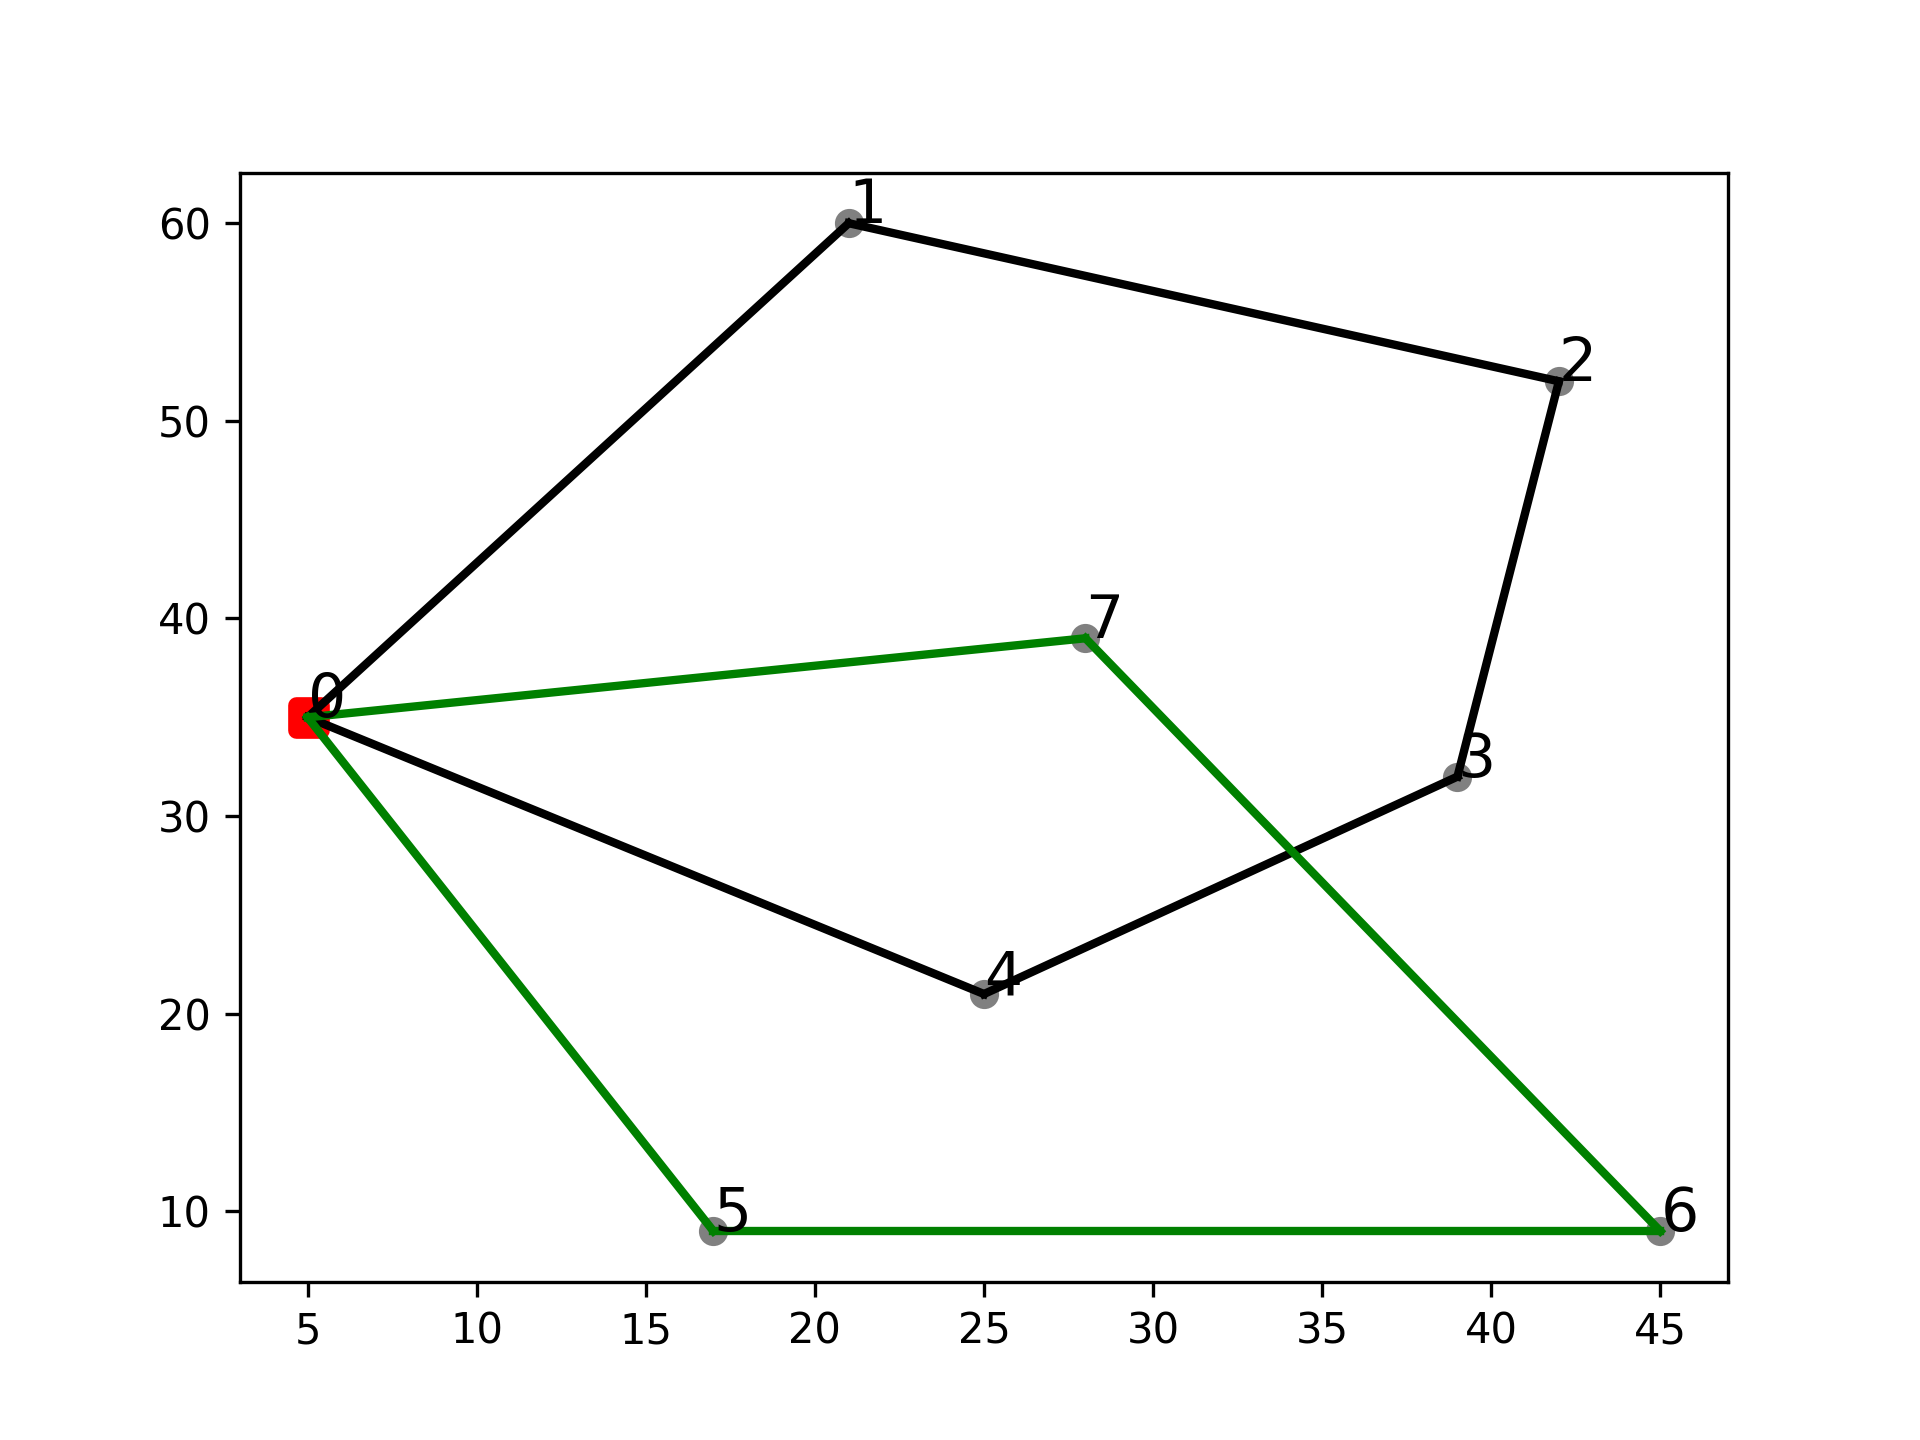
\includegraphics[width=6cm]{resources/opt2/before.png}
    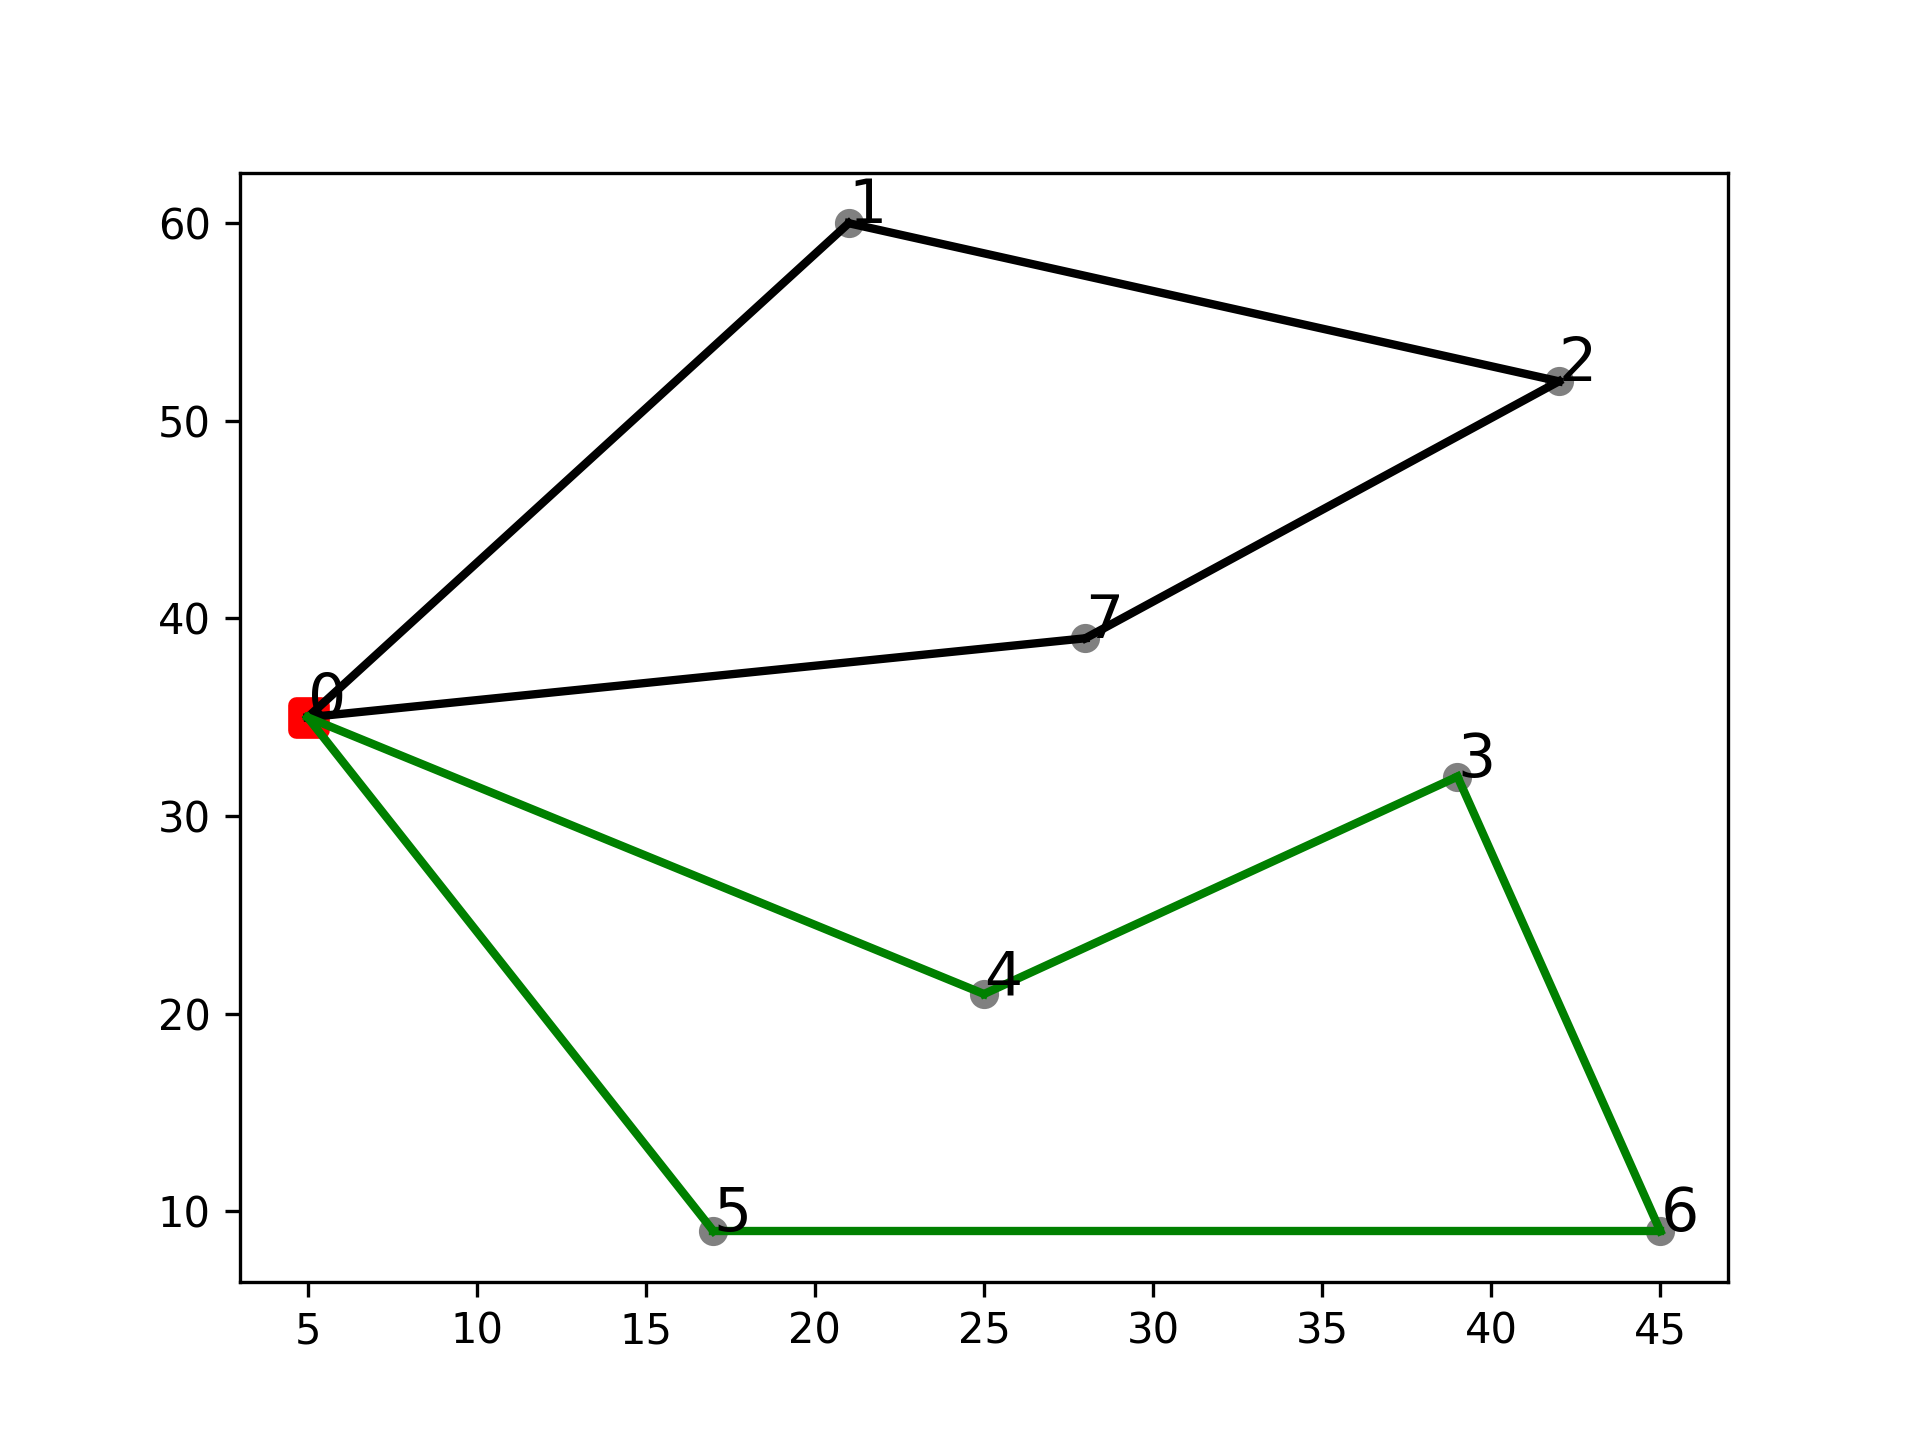
\includegraphics[width=6cm]{resources/opt2/after.png}
    \caption{Ejemplo de intercambio de subrutas. Se intercambia los nodos finales de la ruta negra (3 y 4) a la ruta verde y el nodo final de la ruta verde (7) a la ruta negra.}
    \label{opt2example}
  \end{figure}

  OPT2 logró una mejora en las soluciones respecto a la fase de construcción en todos los casos como se detallará en la sección de resultados. Sin embargo habían casos en que esta transformación no era suficiente ya que las soluciones eran parecidas a las óptimas a menos de algunos clientes que debían ser movidos de una ruta a otra u el órden de los clientes dentro de cada ruta.

  \subsubsection*{Insertion}

  Para contemplar algunas falencias de OPT2, se implementó la búsqueda que llamaremos Insertion. Lo que hace es dada dos rutas A y B, intenta insertar un cliente de A en B de manera de reducir la suma de los costos de ambas rutas.

  \subsection*{Ajuste de parámetros}

  Como se mencionó anteriormente, el ajuste del GRASP se realizó comparando contra las instancias de 25 nodos de Solomon.
  
  Los parámetros del GRASP a ajustar son, a grandes rasgos:

  \begin{enumerate}
    \item {Los que determinan el costo de un movimiento. Estos son los $W_d, W_t y W_w$ de la ecuación \ref{eq:rclmovecost}}.
    \item {En las búsquedas locales, si hacer {\it first improvement} ó {\it best improvement} en cada una y a nivel general. Recordemos que las búsquedas locales implementadas genera vecindades sobre un par de caminos, aquí tenemos un nivel de {\it first/best improvement}. Luego a nivel de solución se puede decidir {\it first/best improvement} para el espacio de búsqueda de pares de caminos, es decir si para el primer par de caminos que $X$ búsqueda local encuentra una mejor solución, o para el par de caminos que mejor solución vecina encuentra.}
  \end{enumerate}

  \subsubsection*{Calibración parámetros de costo de movimiento}

  Para calibrar los primeros, se consideraron combinaciones de valores de dichos parámetros que suman 1 y se ejecutaron todas las instancias de prueba. Para determinar las combinaciones, se consideró un conjunto de valores entre 0 y 1. Esto devino en 22 posibles configuraciones que fueron ejecutadas en el cluster, esta ejecución no incluyó la búsqueda local.

  Para evaluar la mejor asignación se tuvieron datos sobre las 18 instancias de prueba y 22 ejecuciones. El primer paso fué descartar las ejecuciones que no encontraron soluciones factibles para alguna instancia, dado que no hay una fase de corrección de soluciones no factibles, estas configuraciones dejan mal parado al algorítmo. Esto descartó 4 conjuntos de configuraciones.

  Luego, para obtener una visión a gran escala del desempeño de las configuraciones, se decidió comparar la suma de las 18 soluciones entre configuraciones y compararlas con un histograma. De esto, nos quedamos con las 7 mejores configuraciones cuyo desempeño agregado es similar como se observa en la figura \ref{cmphistogram}.

  Finalmente, calculando el promedio y desviación estándar del error de las soluciones contra las de referencia, se eligió la configuración que minimizaba ambos valores. Esta es: $W_d = 0.7, W_t = 0.1 y W_w = 0.2$.

  \begin{figure}
    \centering
    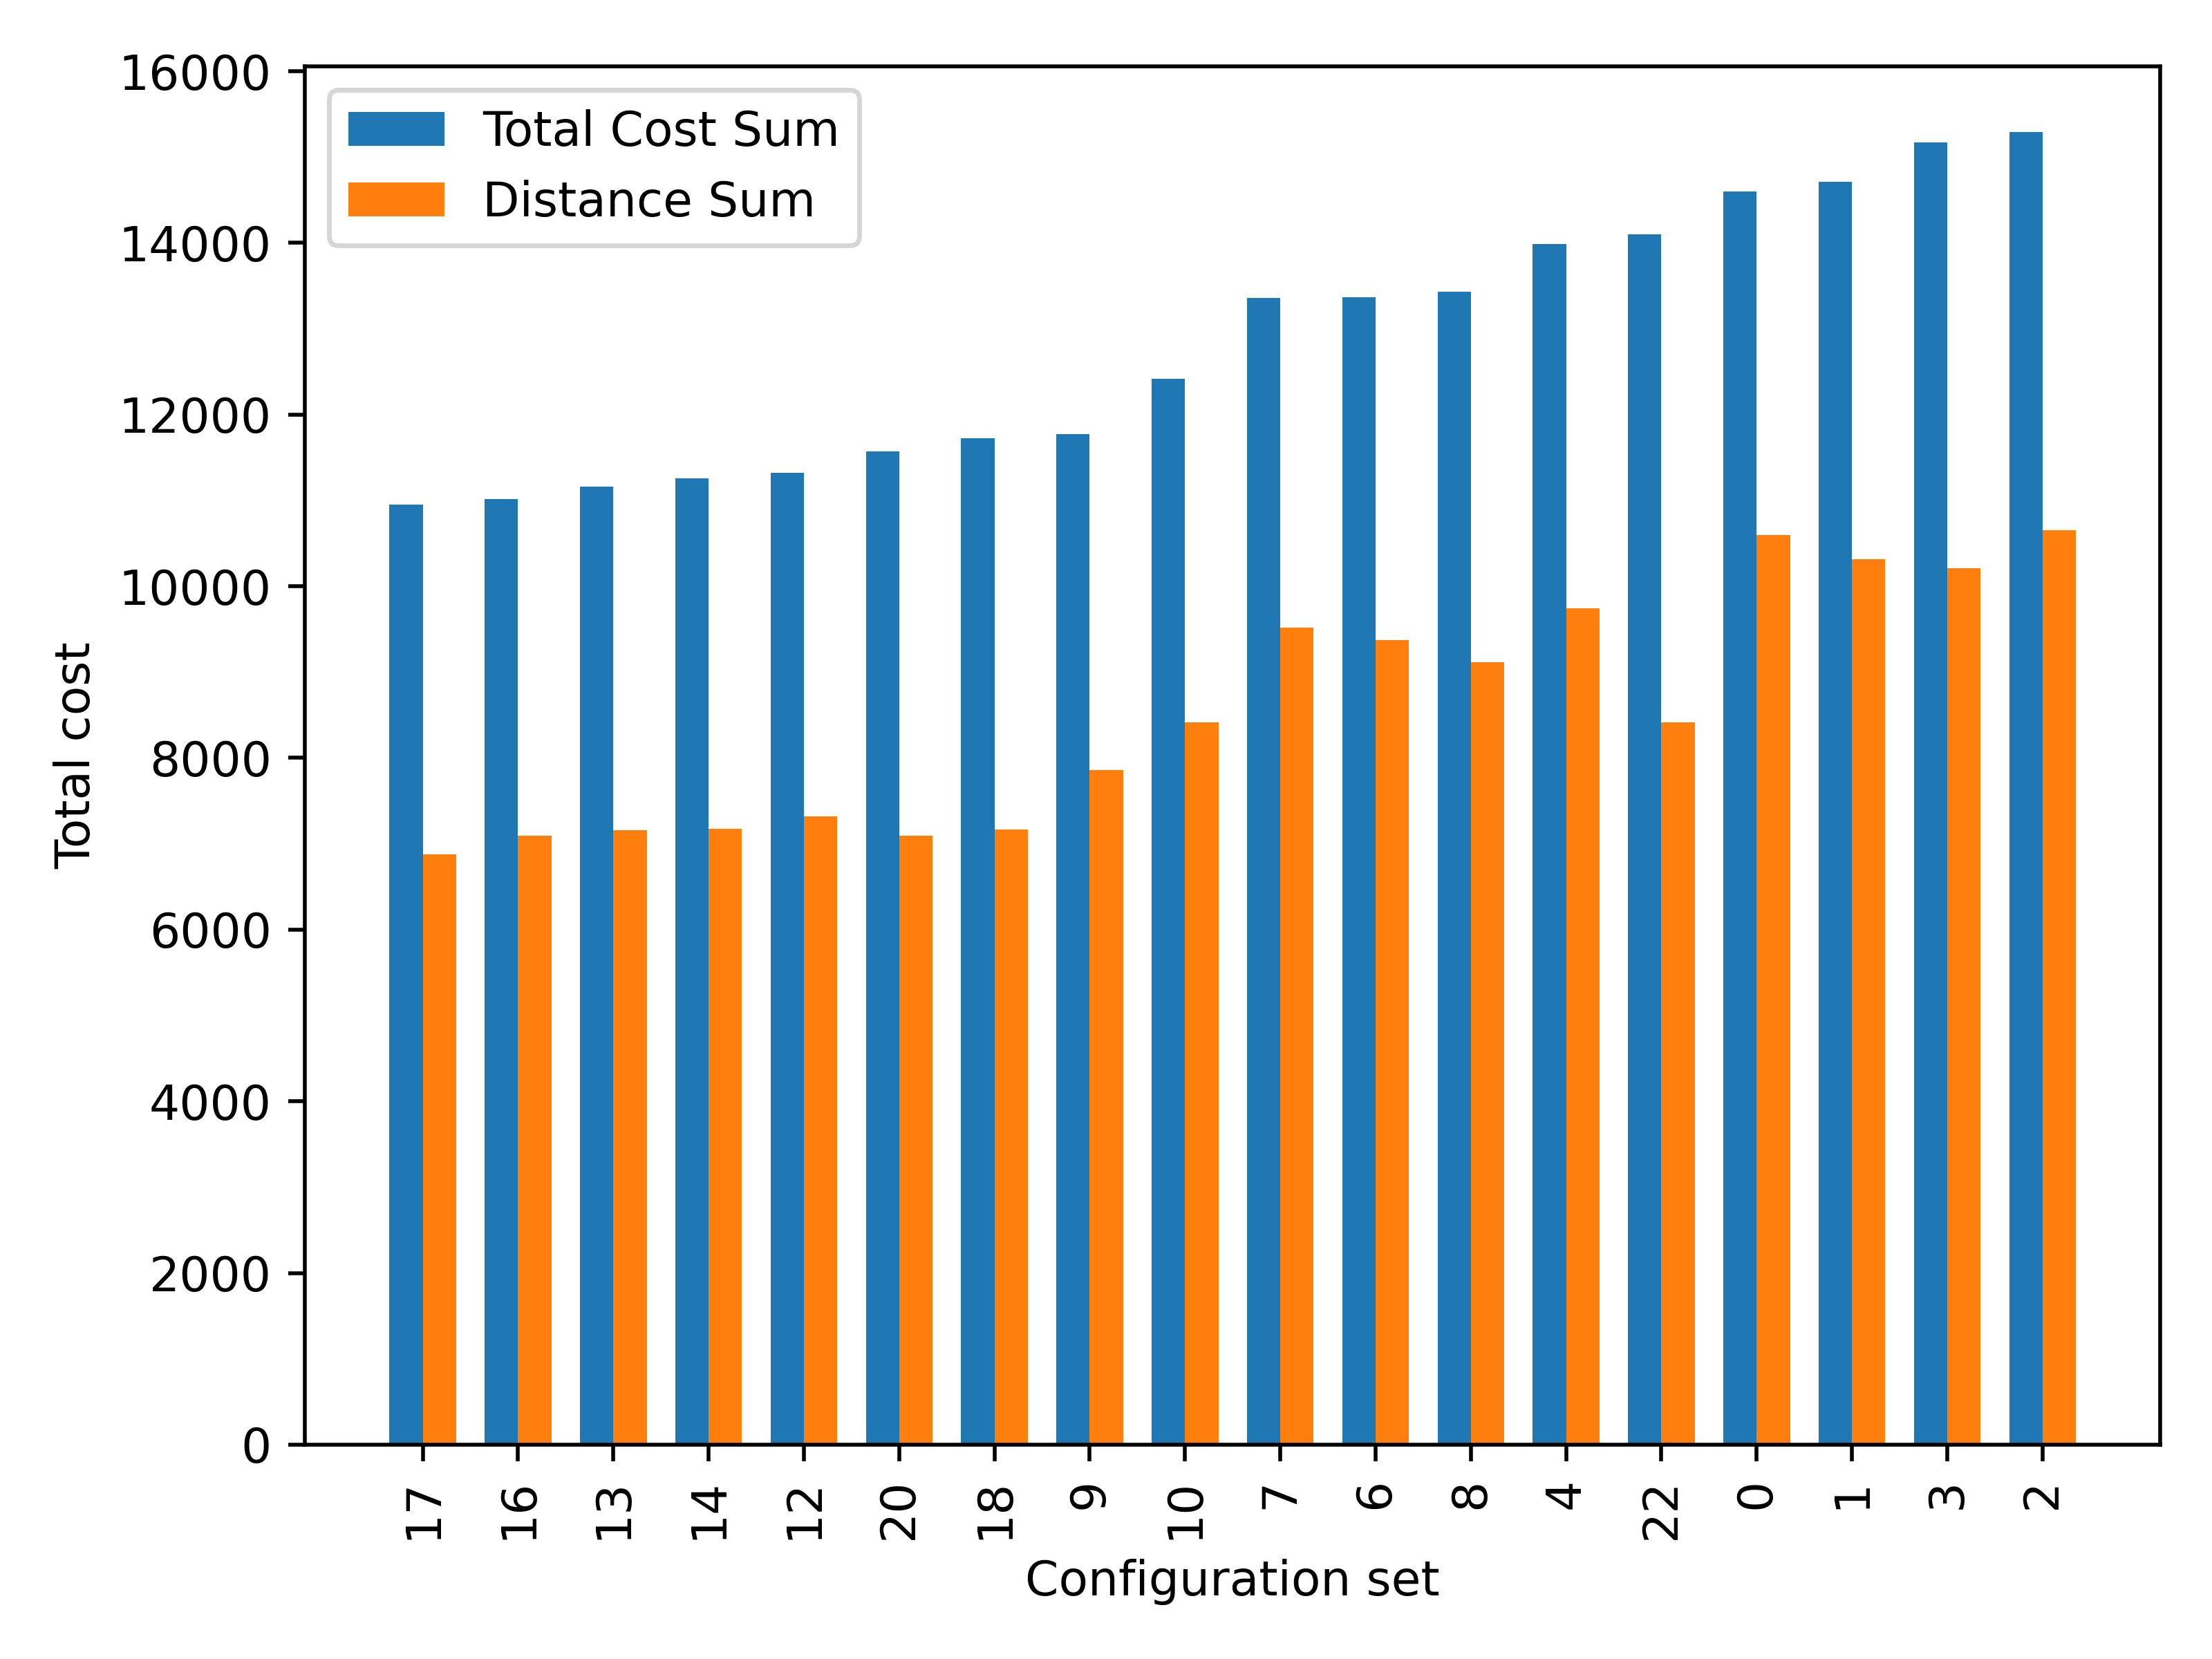
\includegraphics[width=10cm]{resources/tunning/total_cost_histogram_used.png}
    \caption{Histograma donde se compara la suma de los costos de las soluciones encontradas por cada configuración. Se consideran dos factores: el costo total y la distancia. El primero es el valor objetivo, el segundo es un valor que se es deseable que sea mínimo}.
    \label{cmphistogram}
  \end{figure}

  \subsubsection*{Calibración de búsquedas locales}

  Con los parámetros de la sección anterior ya configurados, se procedió a investigar el comportamiento de la búsqueda local respecto a {\it first/best improvement}. Se generaron las ocho combinaciones posibles de los tres parámetros booleanos y se realizaron las ejecuciones tomando $LocalSearchMaxiter = 1000$ (ver \ref{grasp}). Como resultado no se vió mayor diferencia en ninguna de las ejecuciones. Ocurrieronme dos explicaciones para esto: que el tamaño de las instancias es demasiado chico para podes; que la cantidad de iteraciones $LocalSearchMaxiter$ haga que el se comporten igual. Se decidió elegir la configuración mas rápida, es decir {\it first improvement} par las tres variables.

  \section*{Resultados}

  \section*{Conclusión}

  \section*{Trabajo a futuro}

  \subsection*{Mejor consideración de movimientos por vehículo}
  
  En la implementación de este trabajo, la cantidad de movimientos por vehículo a incluir en la RCL es un parámetro del modelo. Se podría tomar enfoque mas inteligente y tomar una cantidad variable de movimientos dependiendo que tan buenos sean estos, por ejemplo, de la misma manera que se construya la RCl.

  \section*{Implementación}

  \section*{Referencias}

  \begin{enumerate}
    \item{\label{jiang} Jun Jiang, Kien Ming Ng, Kim Leng Poh, Kwong Meng Teo (2014). Vehicle routing problem with a heterogeneous fleet and time windows}
    \item{\label{inco} Lucía Barrero, Rodrigo Viera, Franco Robledo, Claudio Risso, Sergio Nesmachnow, Andrei Tchernykh (2020). Exact resolution of the Vehicle Routing Problem with Flexible Time Windows}
    \item{\label{solomon} Solomon, M. M. (1985). Algorithms for the vehicle routing and scheduling problems with time window constraints}
    \item{\label{repo} Repositorio de la implementación del GRASP. \url{https://github.com/joaquinco/mor-proj}}
  \end{enumerate}
\end{document}
